\documentclass[11pt,journal,compsoc]{IEEEtran}

\usepackage[utf8]{inputenc}
\usepackage{xcolor}
\newcommand\todo[1]{\textcolor{red}{[#1]}}

\usepackage{listings}

\usepackage{tikz}
\usetikzlibrary{shapes,arrows}

\renewcommand\appendix{\par
  \setcounter{section}{0}
  \setcounter{subsection}{0}
  \setcounter{figure}{0}
  \setcounter{table}{0}
  \renewcommand\thesection{Appendix \Alph{section}}
  \renewcommand\thefigure{\Alph{section}\arabic{figure}}
  \renewcommand\thetable{\Alph{section}\arabic{table}}
}
\newcommand{\HRule}{\rule{\linewidth}{0.5mm}}

% *** CITATION PACKAGES ***
%
\ifCLASSOPTIONcompsoc
  % IEEE Computer Society needs nocompress option
  % requires cite.sty v4.0 or later (November 2003)
  % \usepackage[nocompress]{cite}
\else
  % normal IEEE
  % \usepackage{cite}
\fi

% Define block styles
\tikzstyle{initBlock} = [draw, draw, fill=blue!20, 
    text width=6.5em, text badly centered, node distance=3cm, inner sep=0pt, minimum width=7em, minimum height=5em]
\tikzstyle{block} = [rectangle, draw, fill=green!20, text centered,text width=5em, rounded corners, minimum height=4em]
\tikzstyle{largerblock} = [rectangle, draw, fill=green!20,text centered, rounded corners, minimum height=4em]    
\tikzstyle{line} = [draw, -latex']
\tikzstyle{cloud} = [draw, ellipse,fill=blue!20, node distance=3cm,
    minimum height=2em]


% *** GRAPHICS RELATED PACKAGES ***
%
\ifCLASSINFOpdf
  % \usepackage[pdftex]{graphicx}
  % declare the path(s) where your graphic files are
  % \graphicspath{{../pdf/}{../jpeg/}}
  % and their extensions so you won't have to specify these with
  % every instance of \includegraphics
  % \DeclareGraphicsExtensions{.pdf,.jpeg,.png}
\else
  % or other class option (dvipsone, dvipdf, if not using dvips). graphicx
  % will default to the driver specified in the system graphics.cfg if no
  % driver is specified.
  % \usepackage[dvips]{graphicx}
  % declare the path(s) where your graphic files are
  % \graphicspath{{../eps/}}
  % and their extensions so you won't have to specify these with
  % every instance of \includegraphics
  % \DeclareGraphicsExtensions{.eps}
\fi

% *** TITLE/SUBJECT/AUTHOR/KEYWORDS INFO BELOW!!           ***
\newcommand\MYhyperrefoptions{bookmarks=true,bookmarksnumbered=true,
pdfpagemode={UseOutlines},plainpages=false,pdfpagelabels=true,
colorlinks=true,linkcolor={black},citecolor={black},urlcolor={black},
pdftitle={Bare Demo of IEEEtran.cls for Computer Society Journals},%<!CHANGE!
pdfsubject={Typesetting},%<!CHANGE!
pdfauthor={Michael D. Shell},%<!CHANGE!
pdfkeywords={Computer Society, IEEEtran, journal, LaTeX, paper,
             template}}%<^!CHANGE!

% correct bad hyphenation here
\hyphenation{op-tical net-works semi-conduc-tor}


\begin{document}
%
% paper title
\title{Artificial Intelligence and Decision Systems: Assignment \#3}


\author{D. Monteiro (70125),$^\dagger$\thanks{$^\dagger$ MSc. student of Aerospace Engineering, Instituto Superior Técnico, Lisbon, Portugal. Student Nr: $70125$}, R.F. Santos (69278)$^\ddagger$\thanks{$^\ddagger$ MSc. student of Aerospace Engineering, Instituto Superior Técnico, Lisbon, Portugal. Student Nr: $69278$}\\[.2 cm]
\textit{University of Lisbon, Lisbon, Portugal}}% <-this % stops a space
     

% for Computer Society papers, we must declare the abstract and index terms
% PRIOR to the title within the \IEEEtitleabstractindextext IEEEtran
% command as these need to go into the title area created by \maketitle.
% As a general rule, do not put math, special symbols or citations
% in the abstract or keywords.
\IEEEtitleabstractindextext{%
\begin{abstract}
In this assignment, a program was made in python to prove propositional logic theorems based on the resolution principle.
\end{abstract}

% Note that keywords are not normally used for peerreview papers.
\begin{IEEEkeywords}
resolution theorem, propositional logic, clausal normal form, CNF, knowledge base.
\end{IEEEkeywords}}


% make the title area
\maketitle

%\IEEEdisplaynontitleabstractindextext
% \IEEEdisplaynontitleabstractindextext has no effect when using
% compsoc under a non-conference mode.


% For peer review papers, you can put extra information on the cover
% page as needed:
% \ifCLASSOPTIONpeerreview
% \begin{center} \bfseries EDICS Category: 3-BBND \end{center}
% \fi
%
% For peerreview papers, this IEEEtran command inserts a page break and
% creates the second title. It will be ignored for other modes.
\IEEEpeerreviewmaketitle

\section{Introduction}

\IEEEPARstart{T}{he} aim of the present short report is to describe the results obtained for the Assignment \#3 which aimed the creation of a resolution-based theorem prover for propositional logic. This assignment is a continuation of the previous one, where a Clausal Normal Form (CNF) converter was made. This way, it is assumed that the given knowledge base and sentence to prove is already in the CNF form.

This report will start with the discussion of the resolution theorem prover, particularly its algorithm and implementation. After that, there will be some complementary remarks and conclusions.

The code was made using \textsc{Python} v2.7 released for \textsc{Unix} operating systems.

\hfill 
 
\hfill \today

\section{Resolution Theorem Prover}
The resolution theorem enables to prove propositional logical sentences given an assumed knowledge base.  In other words, it allows to conclude whether a propositional formula is satisfiable or unsatisfiable under that knowledge base. The main idea behind this technique of logical inference is to prove the unsatisfiability of the negated sentence which one aims to prove. This form of theorem proving is generally referred as refutation.\\
The implementation of the theorem prover in this assignment followed the algorithm presented as a block diagram in \ref{app:init_resolution}. Initially, the algorithm uses the CNF converter to generate a list of disjunctions for both the knowledge base (KB) and sentence to prove ($\alpha$). After that step, the reasoning was to investigate the validity of each clause in $\alpha$ independently. While each clause provides a \texttt{True} outcome, the routine keeps evaluating the following clauses until a point where one clause is not satisfied by the knowledge base or there are no more clauses to evaluate. The result obtained would be then \texttt{False} or \texttt{True}, respectively. This algorithm proved to be efficient observing that when a \texttt{False} is detected, the routine stops since the outcome of any other clause is irrelevant for the final result.\\
As suggested in the assignment description, the unit preference heuristic was applied. With this strategy the algorithm gives preference to resolutions where at least one of the clauses is a single literal. This way it is always ensured that for any conclusive resolution the outcome is always a shorter clause. This strategy clearly helps to reach a conclusion faster, since our algorithm seeks for resolutions where a literal and its negated counterpart are involved, such that a final conclusion about the clause to prove can be arisen. It is also important to note that the application of this heuristic does not fail because with the inclusion of the clause to prove $\alpha_i$ in the knowledge base (see \ref{app:init_resolution}), it is guaranteed the presence of unit clauses even if KB does not contain any.
In order to better understand the application of the unit preference heuristic and the reasoning behind the function \texttt{ResolutionLoop(Union)}, its general algorithm is presented here:\\

\small
\noindent\texttt{loop until no new clauses result from any pair of clauses in Union:
\begin{enumerate}
\item for each pair of clauses $C_i$, $C_j$ in Union
\item result = Resolution($C_i$,$C_j$)
\item if result contains the empty clause, return True
\item elseif result is a shorter clause, add result to Union and pop $C_j$
\end{enumerate}
}
\normalsize
Note that in step \texttt{4)}, the \texttt{pop} is possible since in our algorithm the \texttt{$C_i$} clause is always a unit clause due to the heuristic applied. This means that the result if conclusive (i.e. a shorter clause) is a simplification of \texttt{$C_j$} and therefore the latter can be withdrawn from \texttt{Union}. \todo{better explain resolution}



\section{Complementary Remarks}

\subsection{User Interface}

To run the program, the user should insert the file name from where he wants to load a list of sentences. In this file, the sentences must have the same form as they had in the inputs for the previous assignment.

To run the program in a Linux based operative system, the following command should be inserted in the terminal:

\noindent
\begin{lstlisting}[language=bash]
  $ python resolution-prover.py [file]
\end{lstlisting}

Where \texttt{[file]} must be replaced by the filename.

The program starts listing all the sentences read from the file and the user is asked to select the Knowledge Base and the sentence to be proven.

After this, a menu is presented with several options. The first one lists the knowledge base and sentence selected previously. The second option applies the resolution algorithm and outputs \texttt{True} when the sentence can be proven from the KB and \texttt{False} otherwise. The third option does the same as the second, but also asks for the name of the file where the user wants to save the result.

The fourth option applies the algorithm listing step by step the operations executed. The result of the application of the unit preference heuristic is shown on the terminal as well as the result of the application of the resolution algorithm to two clauses from the knowledge base.

The fifth option does the same as the fourth, but saves the output to a file, and the last option exits the program.


\subsection{Discussion}

While developing the code for this assignment, one of the aspects taken into account was to try to provide a readable and clean output. For this end, the function developed in the previous assignment to convert the sentences to a more human readable way was used to present the sentences read from the file. Besides that, the step by step resolution just presented as an output the result of the application of resolution when the list of clauses was changed.

The resolution-based theorem prover developed was tested for several different knowledge bases, with different degrees of complexity, and proved to behave efficiently and provide correct results for all those cases.



% references section

% can use a bibliography generated by BibTeX as a .bbl file
% BibTeX documentation can be easily obtained at:
% http://www.ctan.org/tex-archive/biblio/bibtex/contrib/doc/
% The IEEEtran BibTeX style support page is at:
% http://www.michaelshell.org/tex/ieeetran/bibtex/
%\bibliographystyle{IEEEtran}
% argument is your BibTeX string definitions and bibliography database(s)
%\bibliography{IEEEabrv,../bib/paper}
%
% <OR> manually copy in the resultant .bbl file
% set second argument of \begin to the number of references
% (used to reserve space for the reference number labels box)
\begin{thebibliography}{1}

\bibitem{book}
S.~Russell and P.~Norvig, \emph{Atificial Intelligence - A Modern Approach}, 3rd~ed.\hskip 1em plus
  0.5em minus 0.4em\relax Pearson, 2010.

\end{thebibliography}

%\newpage
\onecolumn

%%%%%%%%%%%%%%%%%%%%%%

%% APPENDIX

%%%%%%%%%%%%%%%%%%%%%
\appendix
\section{Resolution Theorem Prover Algorithm - Function \texttt{init\_resolution(KB,$\alpha$,Flag,Flag)}} \label{app:init_resolution}
\vfill
\begin{figure}[h]
\centering
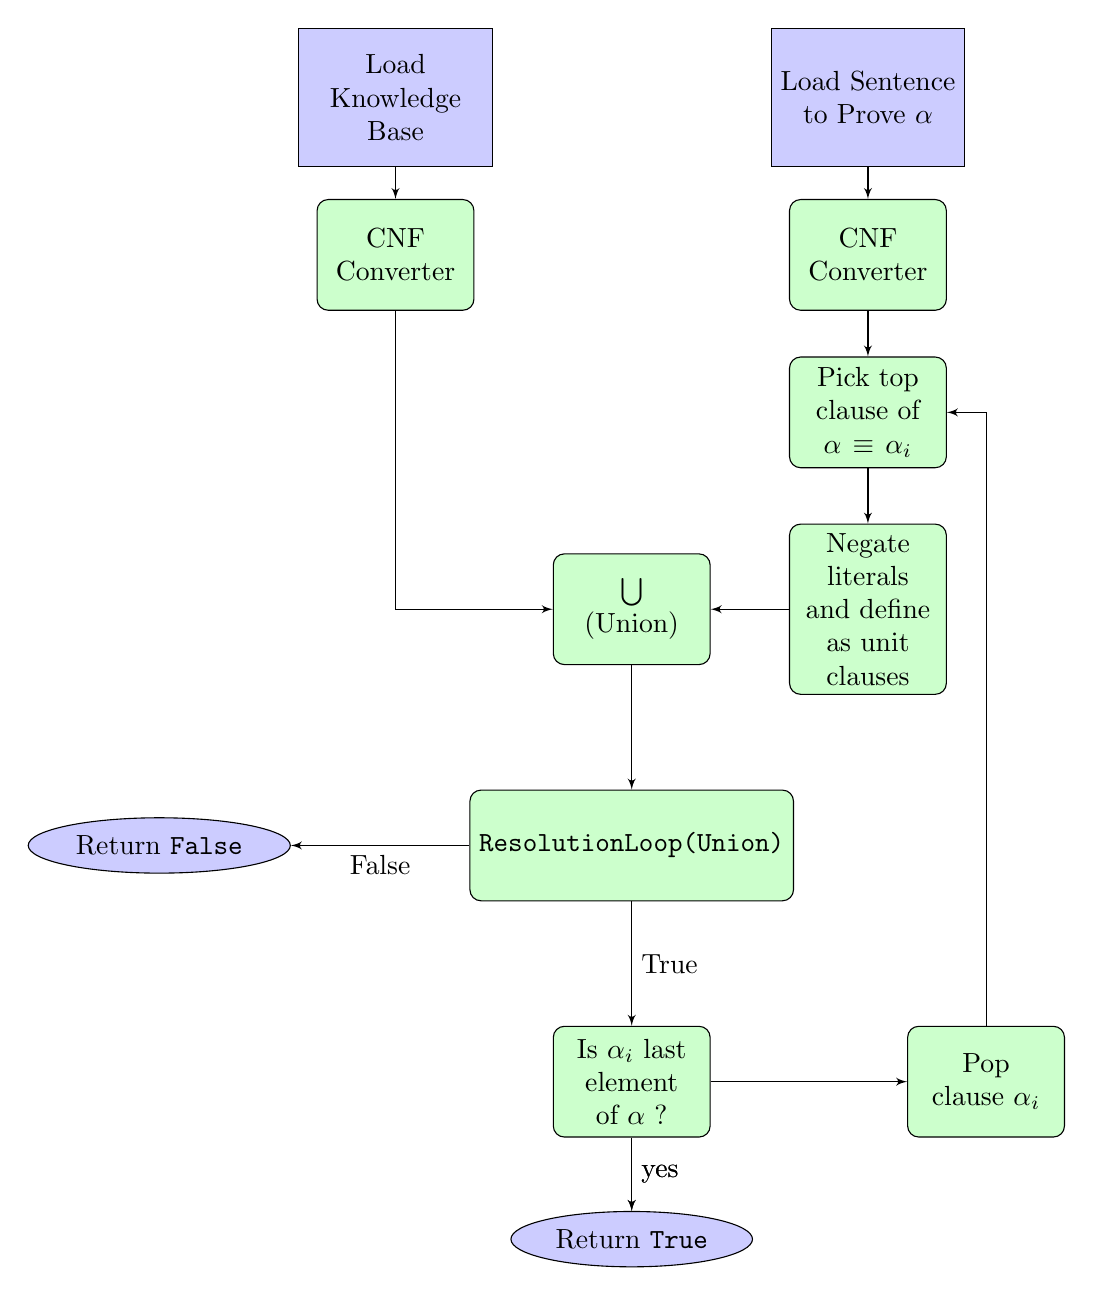
\begin{tikzpicture}[node distance = 2cm, auto]
    % Place nodes
    \node [initBlock] (kb) {Load Knowledge Base};
    \node [initBlock, right of=kb,node distance =6cm] (st) {Load Sentence to Prove $\alpha$};
    \node [block, below of=kb] (CNF1) {CNF Converter};
    \node [block, below of=st] (CNF2) {CNF Converter};
    \node [block, below of=CNF2] (pickClause) {Pick top clause of $\alpha \equiv\alpha_i$};
    \node [block, below of=pickClause,node distance=2.5cm] (negateLiterals) {Negate literals and define as unit clauses};
    \node [block, left of=negateLiterals,node distance=3cm] (union) {$\bigcup$\\(Union)};
    \node [largerblock, below of=union,node distance=3cm] (resolution) {\texttt{ResolutionLoop(Union)}};
    \node [cloud, left of=resolution,node distance=6cm] (returnFalse) {Return \texttt{\textbf{False}}};
    \node [block, below of=resolution,node distance=3cm] (lastElement) {Is $\alpha_i$ last element of $\alpha$ ?};
    \node [block, right of=lastElement,node distance=4.5cm] (pop) {Pop clause $\alpha_i$};
    \node [cloud, below of=lastElement,node distance=2cm] (returnTrue) {Return \texttt{\textbf{True}}};
    %\node [cloud, right of=sentatomic, node distance=6cm] (return) {return};
 
	
    % Draw edges
    \path [line] (kb) -- (CNF1);
    \path [line] (CNF1) |- (union);
    \path [line] (union) -- (resolution);
    \path [line] (resolution) -- node {False} (returnFalse);
	\path [line] (resolution) -- node {True} (lastElement);
	\path [line] (lastElement) -- (pop);
	\path [line] (lastElement) -- node {yes} (returnTrue);
	\path [line] (lastElement) -- node {yes} (returnTrue);
	\path [line] (pop) |- (pickClause);    
    \path [line] (st) -- (CNF2);
     \path [line] (CNF2) -- (pickClause);
     \path [line] (pickClause) -- (negateLiterals);
    \path [line] (negateLiterals) -- (union);
	%\path [line] (sent2) -- node {no} (recursive2);    
	%\path [line] (recursive2) -- (operations);    
    %\path [line] (sent1) -- node {yes} (sent2);
    %\path [line] (sent2) -- node {yes} (operations);
    %\path [line] (operations) -| (return);
\end{tikzpicture}
\end{figure}
\vfill  
\newpage



\vfill  
% biography section
% 
% If you have an EPS/PDF photo (graphicx package needed) extra braces are
% needed around the contents of the optional argument to biography to prevent
% the LaTeX parser from getting confused when it sees the complicated
% \includegraphics command within an optional argument. (You could create
% your own custom macro containing the \includegraphics command to make things
% simpler here.)
%\begin{IEEEbiography}[{\includegraphics[width=1in,height=1.25in,clip,keepaspectratio]{mshell}}]{Michael Shell}
% or if you just want to reserve a space for a photo:


\end{document}


